\documentclass[11pt,a4paper]{article}
\usepackage[utf8]{inputenc}
\usepackage[T1]{fontenc}
\usepackage{lmodern}
\usepackage[margin=2.3cm]{geometry}
\usepackage{graphicx}
\usepackage{booktabs}
\usepackage{array}
\usepackage{amsmath}
\usepackage{hyperref}
\usepackage[most]{tcolorbox}
\usepackage{fancyhdr}
\graphicspath{{docs/figures/}{docs/screens/}}
\hypersetup{colorlinks=true,linkcolor=black,urlcolor=black}

\newtcolorbox{definition}[1][]{colback=white,colframe=black,fonttitle=\bfseries,title=Definition,breakable,#1}
\newtcolorbox{keyconcept}[1][]{colback=white,colframe=black!70,fonttitle=\bfseries,title=Key concept,breakable,#1}
\newtcolorbox{insight}[1][]{colback=black!4,colframe=black!50,fonttitle=\bfseries,title=Insight,breakable,#1}
\newtcolorbox{mistake}[1][]{colback=white,colframe=black!50,fonttitle=\bfseries,title=Found by testing,breakable,#1}
\newcommand{\code}[1]{\texttt{#1}}

\pagestyle{fancy}
\fancyhf{}
\lhead{Semantic Log Analytics for UAV Flight Logs}
\rhead{Sumit Kumar (22CS30056)}
\cfoot{\thepage}
\renewcommand{\headrulewidth}{0.4pt}

\title{\textbf{Semantic Log Analytics for UAV Flight Logs}\\[0.3em]\large A concept explainer for the Advanced Database Management Systems term project}
\author{Sumit Kumar (22CS30056)}
\date{}

\begin{document}
\maketitle
\thispagestyle{fancy}

\begin{abstract}
\noindent This document explains every idea in the project to a reader who has not seen it. Each section gives the plain-English story first and the technical detail (and the measured numbers) second. All figures come from the saved result files under \code{bench/results/}, and each design decision is logged with its evidence in \code{docs/decisions.md}.
\end{abstract}

\tableofcontents
\newpage

% ====================================================================
\section{The Big Picture}
A drone writes a \emph{flight log} on every flight: positions, attitudes, battery voltage, motor commands, plus text messages such as warnings. One log is easy to look at. A \emph{collection} of logs is hard, because the data is three different things at once: a very dense time series (the project corpus has 70.7 million samples from only 300 flights), free text (3,401 events), and vendor-specific names (PX4 and ArduPilot call the same quantity different things).

\begin{keyconcept}
\textbf{Thesis.} Treat the whole log collection as a database problem. One PostgreSQL instance stores the time series compactly, maps vendor fields to shared meanings, searches events by meaning, and lets a language model answer questions in SQL under strict safety rules. Every design choice is justified by a measurement.
\end{keyconcept}

\begin{figure}[h]
\centering
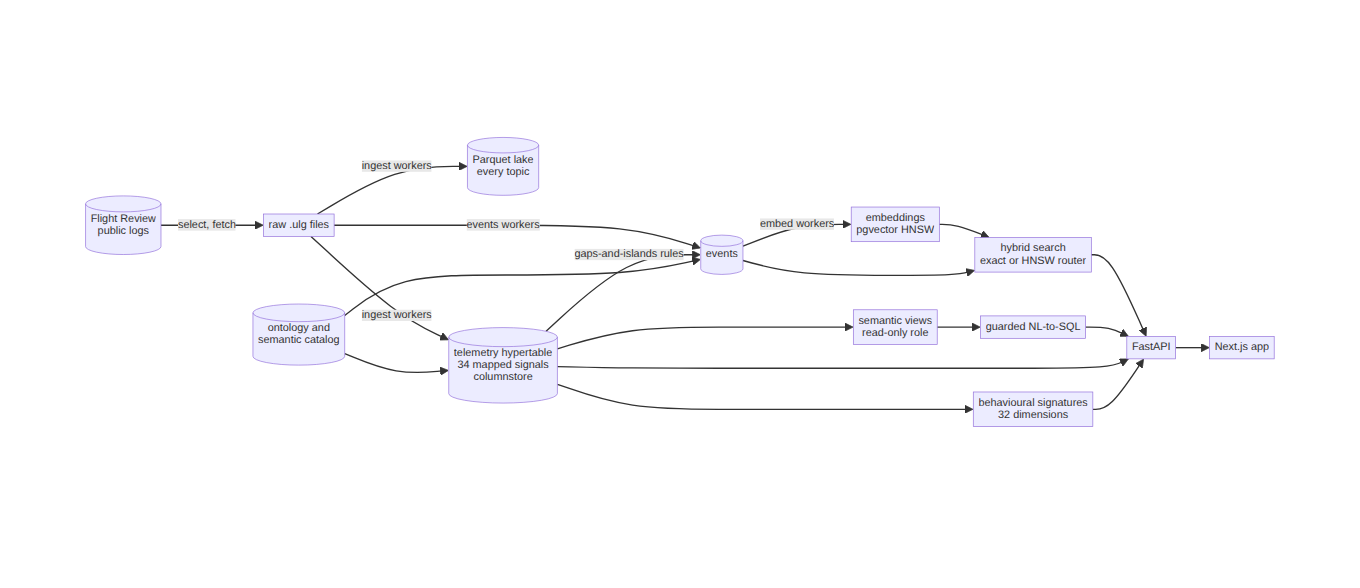
\includegraphics[width=0.95\textwidth]{diagram-architecture.png}
\caption{Architecture: raw logs become a Parquet lake, the canonical telemetry table and events; embeddings and the ontology sit beside them; the application reaches data only through search and guarded read-only views.}
\end{figure}

The work answers four questions: (1) how to store high-rate telemetry and at what cost, (2) which vector index and filtering strategy retrieve events best, (3) whether a model can write safe and correct SQL and what a semantic layer adds, and (4) whether the pipeline survives failure and scales.

\begin{insight}
The project reports negative results as carefully as positive ones: hybrid text-plus-vector search did \emph{not} beat vector-only search, and the semantic views' gain in NL-to-SQL accuracy was \emph{not} statistically significant. Saying so is part of the method.
\end{insight}

% ====================================================================
\section{Core Concepts}
\subsection{Time series, hypertables and chunks}
\emph{Plain English:} a time series is a list of measurements stamped with a time. A \textbf{hypertable} (TimescaleDB) looks like one table but is silently cut into \emph{chunks}, one per time range, so recent data stays small and old data can be treated differently.

\begin{definition}
\textbf{Hypertable}: a logical table partitioned by time into chunks. Here, telemetry uses 7-day chunks.
\end{definition}

\subsection{Columnstore and compression}
\emph{Plain English:} a normal table stores row by row. A columnstore stores each column together, so similar numbers sit side by side and compress extremely well. Reads that need only a few columns, or a few signals, skip the rest.

\begin{definition}
\textbf{Columnstore with \code{segmentby}}: compressed chunk storage where rows are grouped by the \code{segmentby} columns and ordered by \code{orderby}. Here the grouping is (flight, signal), ordered by time.
\end{definition}

\subsection{Embeddings and nearest-neighbour search}
\emph{Plain English:} an embedding turns text into a list of 1,536 numbers so that texts with similar meaning land near each other. Searching by meaning means finding the nearest points. Comparing against every point is exact but slow, so \emph{approximate} indexes trade a little accuracy for speed.
\begin{itemize}
  \item \textbf{HNSW}: a layered graph; you hop from node to nearby node toward the query.
  \item \textbf{IVFFlat}: points are sorted into clusters; you search only the closest few clusters.
  \item \textbf{DiskANN}: a compressed graph built to live mostly on disk (pgvectorscale).
\end{itemize}
\emph{Math:} recall@$k$ is the fraction of the true top-$k$ neighbours the index returns, $\text{recall}@k=|A\cap T|/k$ with $A$ the approximate and $T$ the exact result.

\subsection{Reciprocal rank fusion}
\emph{Plain English:} when two rankers disagree (vector similarity vs keyword match), fuse them by rank, not by raw score, because their scores are not comparable. \emph{Math:} 
\[ \text{RRF}(d)=\sum_{i} \frac{w_i}{k+\text{rank}_i(d)} \]
with weights $w_i$ and a smoothing constant $k$.

\subsection{An ontology as relational tables}
\emph{Plain English:} an ontology is a dictionary of concepts and how they relate. Here it is ordinary tables (concept, relation, vendor field, field mapping) walked with recursive queries.

\subsection{Job queues in a database}
\emph{Plain English:} instead of a separate queue service, the work list lives in a Postgres table. Workers take items with \code{FOR UPDATE SKIP LOCKED}, which means ``take a row nobody else holds''.

% ====================================================================
\section{Contribution 1: Schema and the narrow telemetry table}
\begin{figure}[h]
\centering
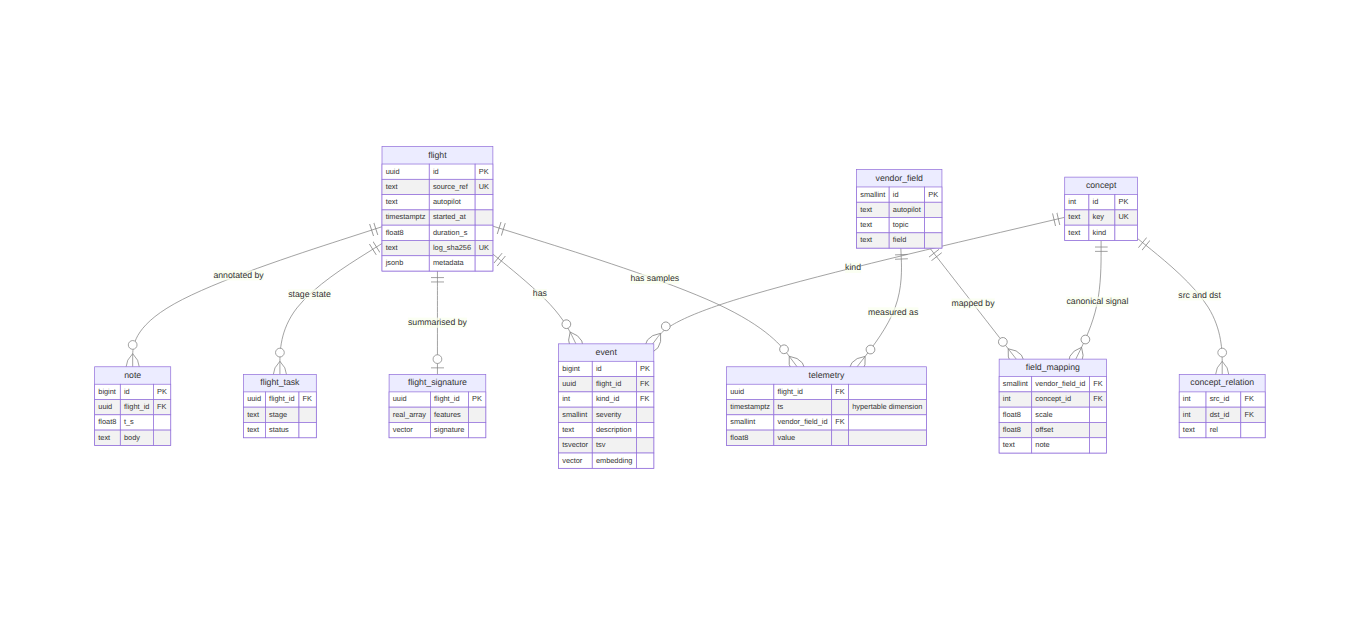
\includegraphics[width=0.85\textwidth]{diagram-er.png}
\caption{Entity-relationship overview.}
\end{figure}

\emph{Plain English:} instead of one column per signal, telemetry has one row per (time, flight, field). It is like a ledger: new kinds of expense add rows, never columns. A new signal, or a whole new autopilot, needs no schema change.

\begin{center}
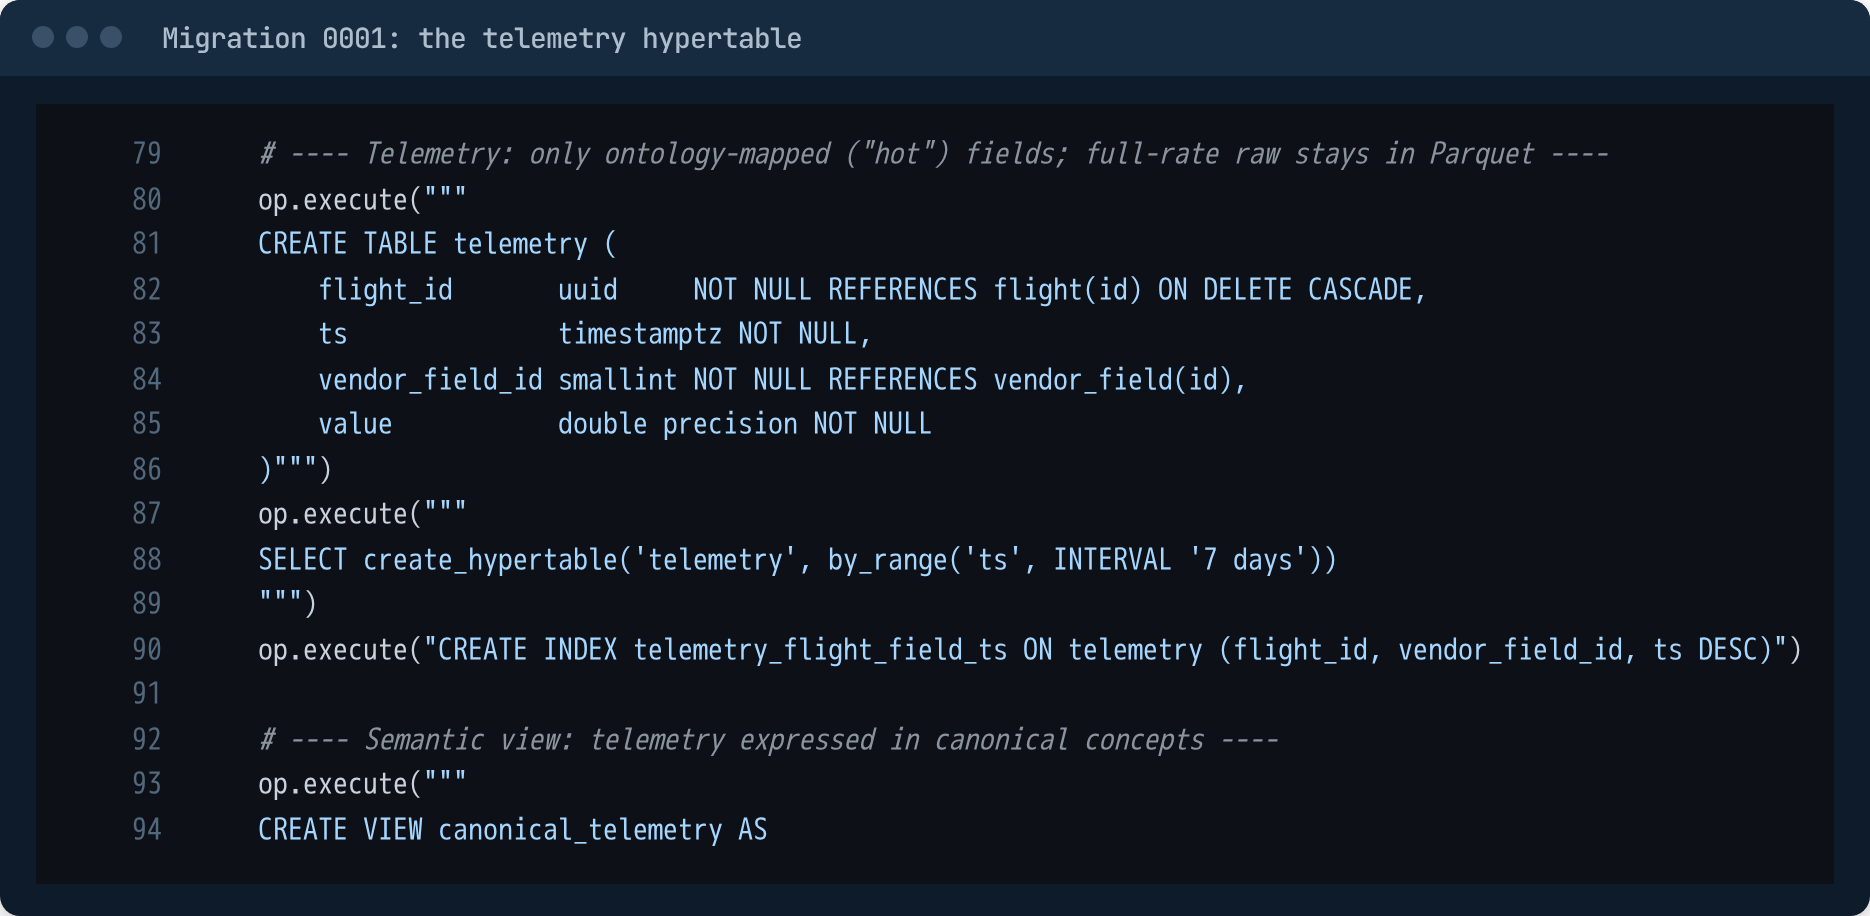
\includegraphics[width=0.7\textwidth]{code-telemetry-ddl.png}
\end{center}

\begin{mistake}
As a plain rowstore the index (7.6 GB) was larger than the table (4.9 GB). That observation is why the columnstore work matters.
\end{mistake}

% ====================================================================
\section{Contribution 2: The semantic layer}
\emph{Plain English:} PX4 might call battery voltage \code{battery\_status.voltage\_v}; ArduPilot calls it something else. The ontology gives both a shared name, \code{battery.voltage}, plus a scale, an offset and a note describing the conversion.

\begin{definition}
\textbf{Semantic layer}: 63 concepts and 55 relations (34 signals, 7 subsystems, 7 failure modes, 15 event kinds) plus a field-mapping table, exposed through documented read-only views.
\end{definition}

\begin{insight}
Five ArduPilot groups were deliberately \emph{not} mapped (vibration, motor outputs, EKF ratios, barometric altitude, flight mode) because their meanings differ. A wrong mapping produces confident wrong answers; a gap produces an honest ``not available''.
\end{insight}

\begin{center}
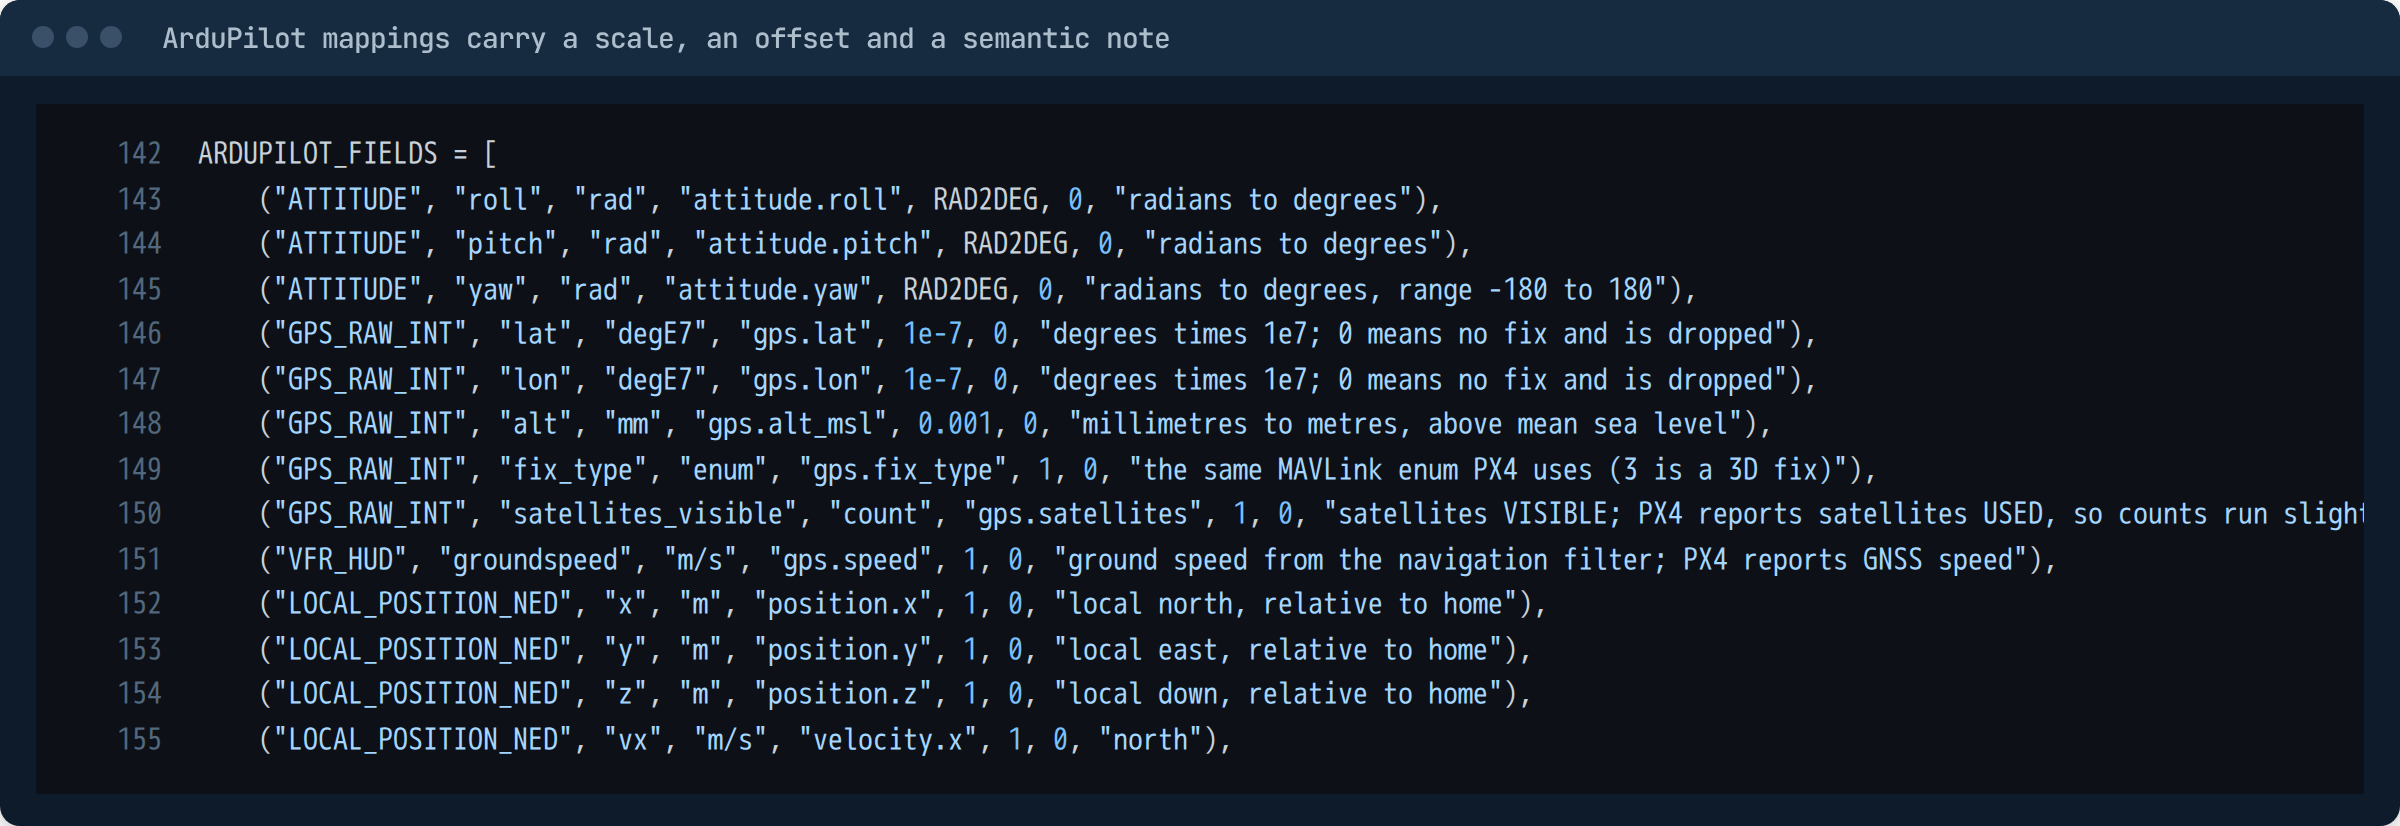
\includegraphics[width=0.85\textwidth]{code-ardupilot-map.png}
\end{center}

\emph{Events.} Events come from log transitions, the failure detector, and \emph{gaps-and-islands} rules over telemetry (window functions that find runs of consecutive abnormal rows). Rules fire only relative to a baseline in the same flight, and near-duplicate messages collapse (3,846 to 3,401).

% ====================================================================
\section{Contribution 3: Pipelines that survive failure}
\begin{figure}[h]
\centering
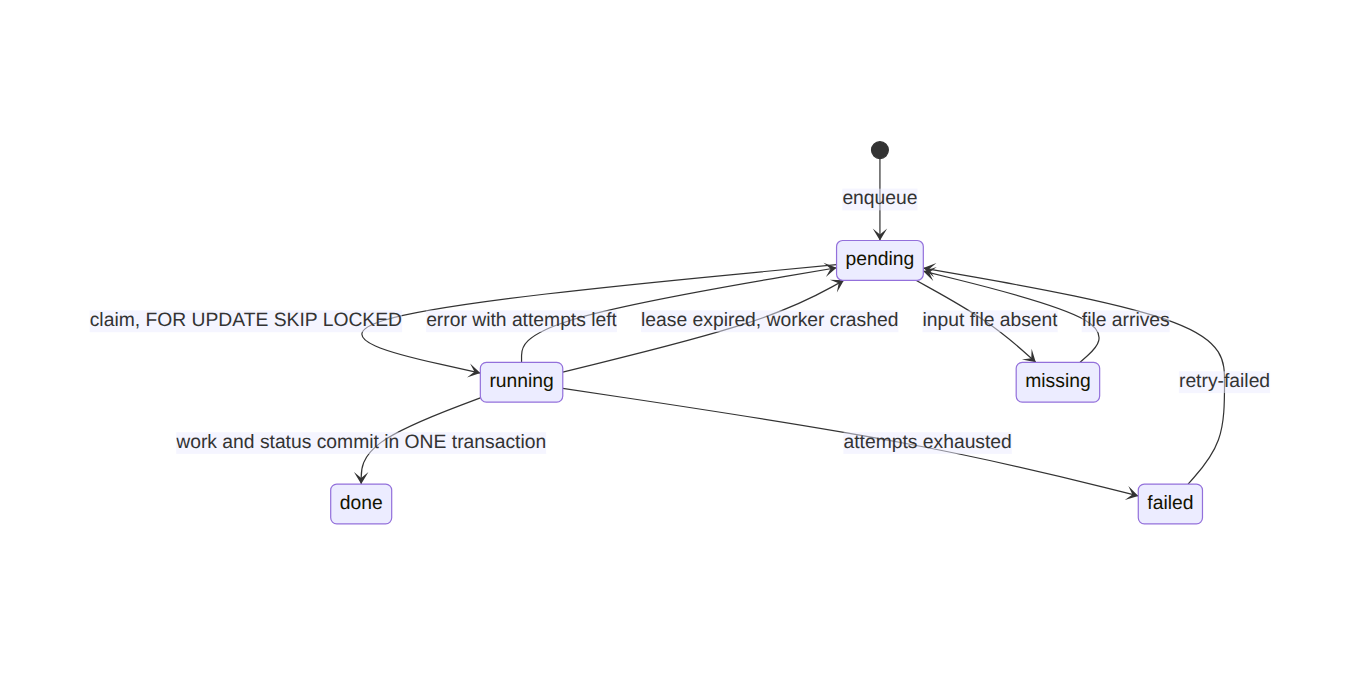
\includegraphics[width=0.7\textwidth]{diagram-queue.png}
\caption{States of a job item.}
\end{figure}

\emph{Plain English:} a deli counter with a ticket machine. Each worker takes a ticket, nobody serves the same ticket twice, and if a worker disappears the ticket returns to the pile when its lease expires.

\begin{keyconcept}
Every batch stage is idempotent, tracked in a job table (status, attempts, last error), claimed with \code{SKIP LOCKED}, failure-isolated, retried, resumable and atomic per item (data and status commit together). To scale you enqueue more items; you do not change code.
\end{keyconcept}

\begin{center}
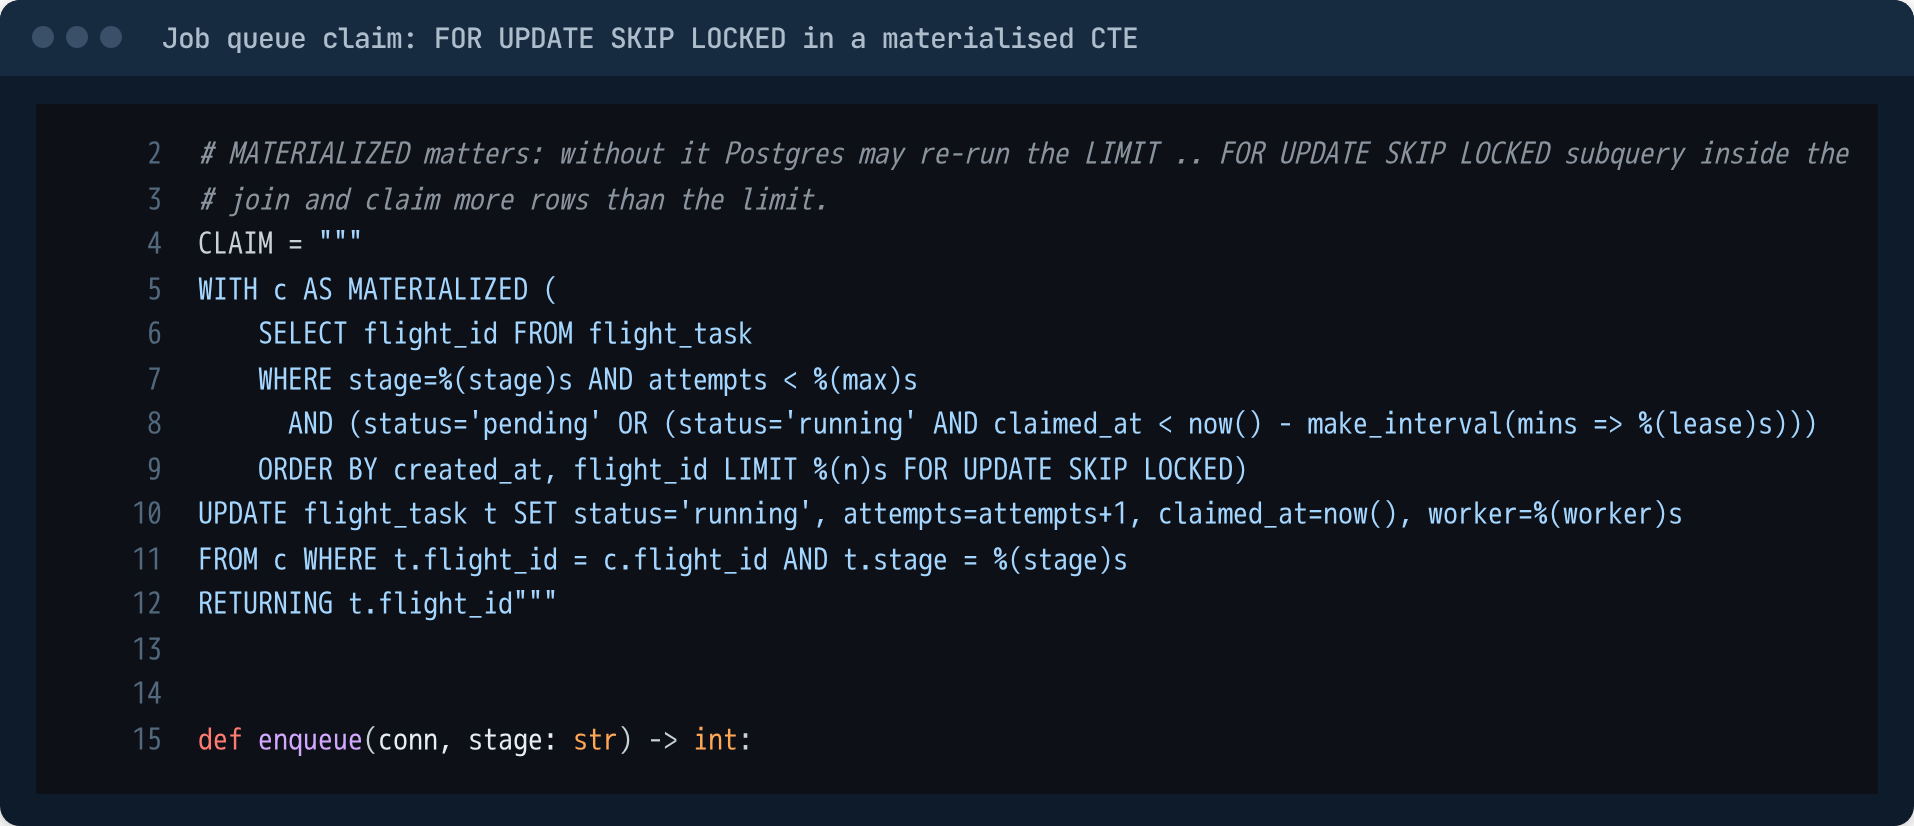
\includegraphics[width=0.75\textwidth]{code-claim.png}
\end{center}

\begin{mistake}
\code{SKIP LOCKED} once claimed 52 rows when asked for 25, because the planner re-ran the subquery. The fix is a \code{MATERIALIZED} CTE. A second bug: a transaction block opened after a read became a \emph{savepoint}, so nothing committed while the run reported success. Both were found by testing from a fresh connection.
\end{mistake}

% ====================================================================
\section{Contribution 4: Hybrid search and the self-routing planner}
\emph{Plain English:} searching events combines meaning (vector), keywords (full text), and hard filters (kind, flight, time). The trap is that pgvector applies a filter \emph{after} it finds neighbours. If a filter keeps one row in a thousand, the index may find 40 neighbours and none pass.

\begin{figure}[h]
\centering
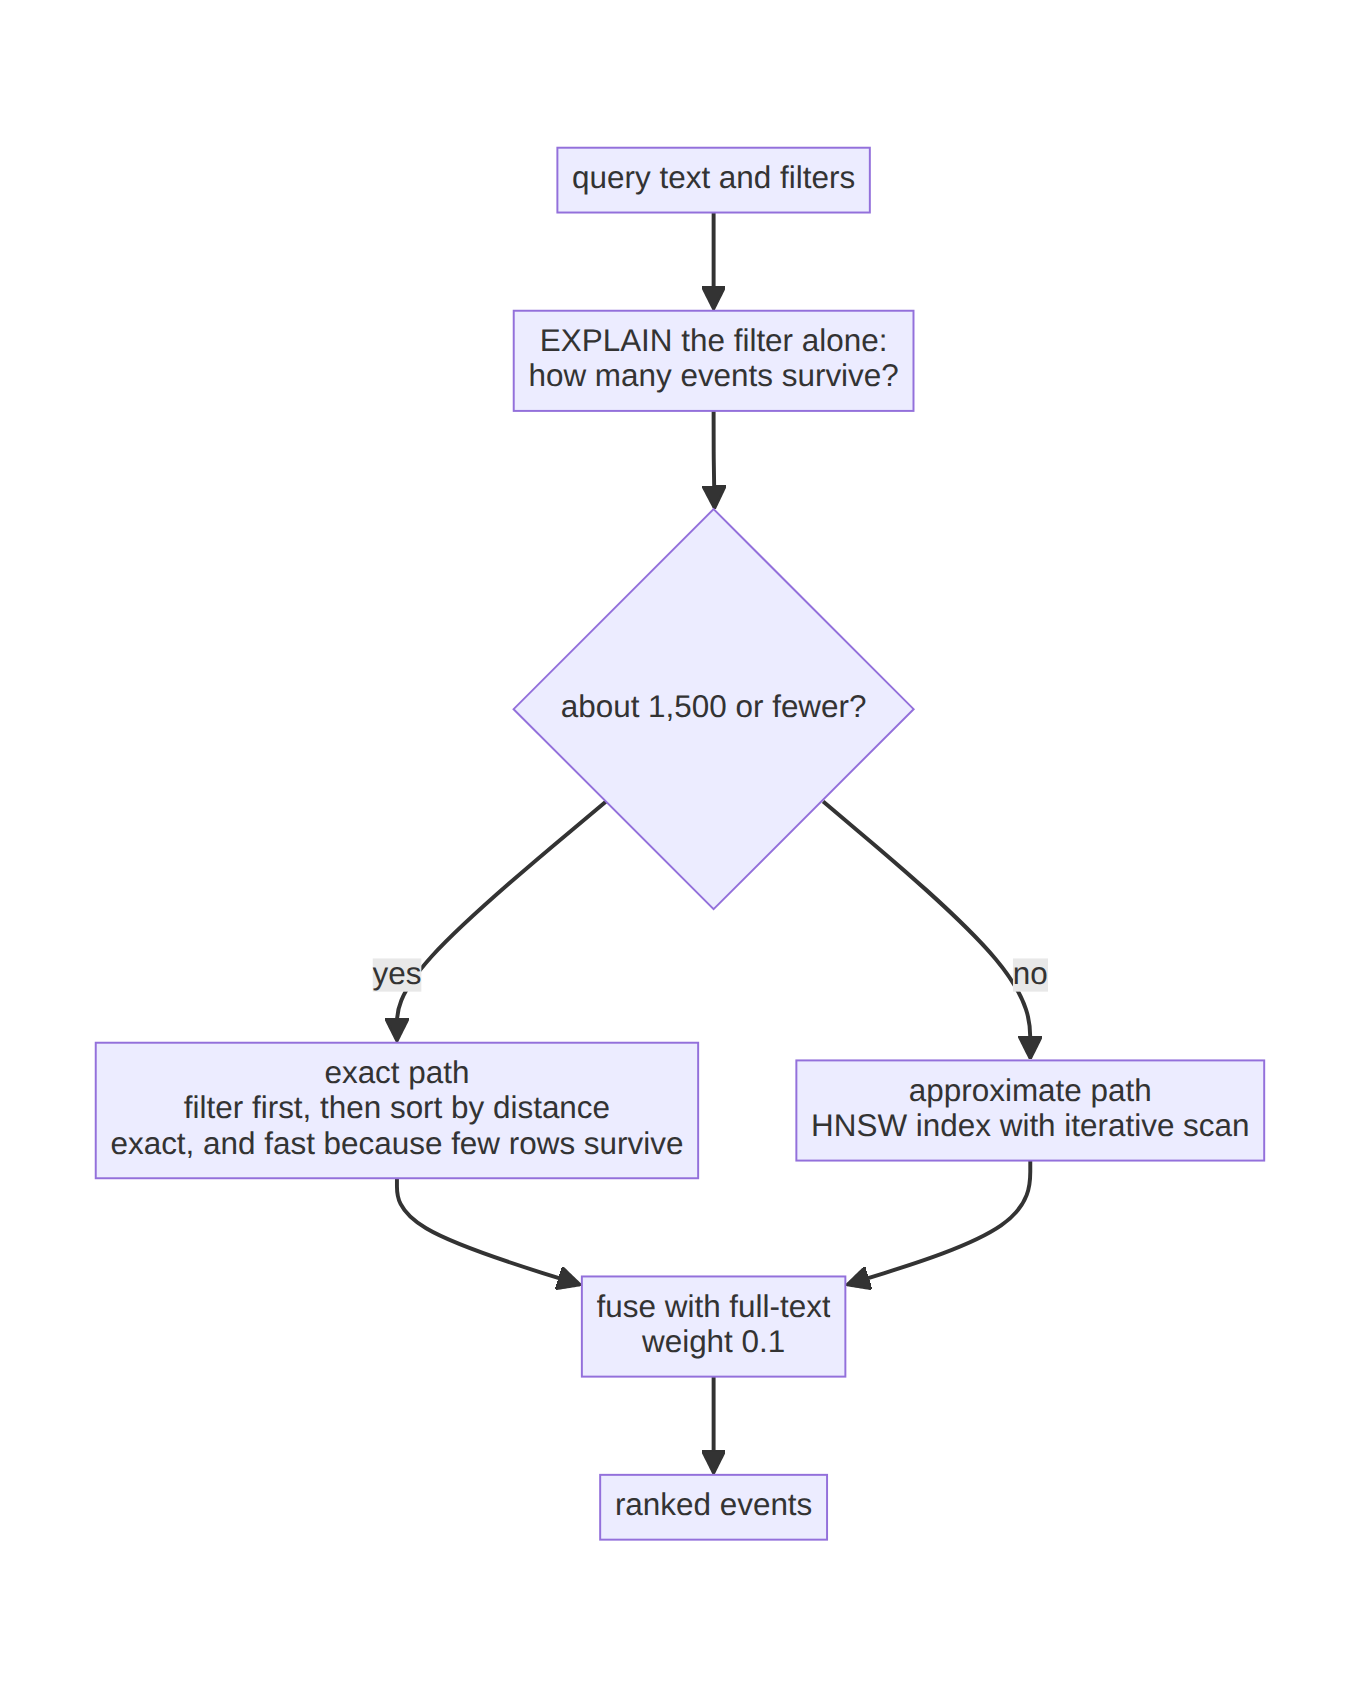
\includegraphics[width=0.45\textwidth]{diagram-router.png}
\caption{Router: estimate the filter's rows with \code{EXPLAIN}; exact path if about 1,500 rows or fewer, HNSW with iterative scan otherwise.}
\end{figure}

\begin{insight}
With both indexes present and a filter keeping 10\% of rows, the planner chose HNSW post-filtering: it returned \textbf{4.0 of 10 rows} with recall 0.37, in 1.6 ms. It is fast and wrong, because a cost model estimates time, not completeness. The router avoids depending on that choice.
\end{insight}

% ====================================================================
\section{Contribution 5: Guarded natural-language SQL}
\emph{Plain English:} a model that writes SQL could, if tricked, read files or run a query that takes the server down. ``It only runs SELECT'' is not a safety boundary. The design uses four independent layers so that defeating one is not enough.

\begin{figure}[h]
\centering
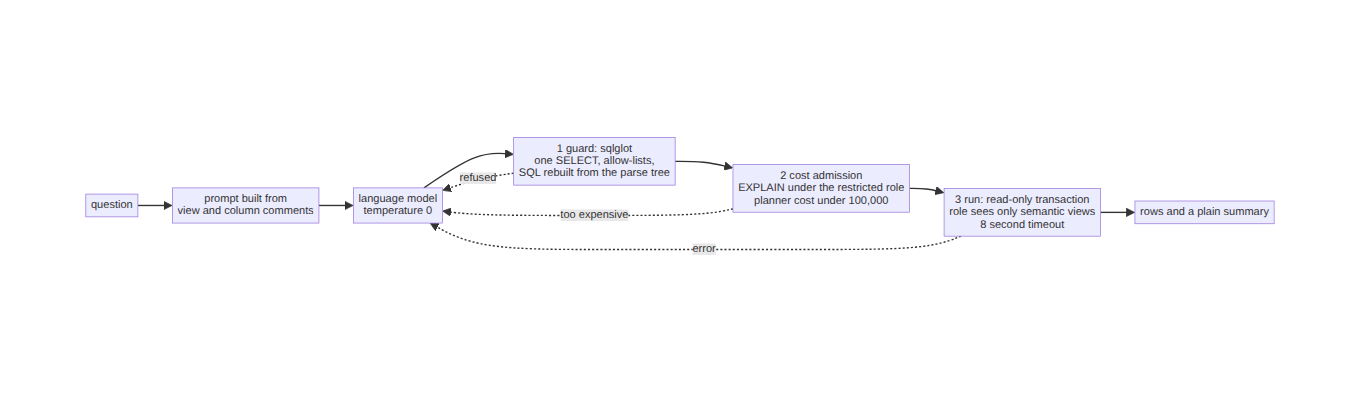
\includegraphics[width=0.9\textwidth]{diagram-guard.png}
\caption{Guard pipeline.}
\end{figure}

\begin{enumerate}
  \item \textbf{Guard} (\code{sqlglot}): exactly one SELECT, allow-listed tables and functions, no nested or recursive WITH; the SQL that runs is \emph{regenerated from the parse tree}, so what was checked is what runs.
  \item \textbf{Role}: a database role that can read only the documented views.
  \item \textbf{Read-only transaction} with an 8 s statement timeout.
  \item \textbf{Cost admission}: \code{EXPLAIN} first; refuse when the planner's estimate exceeds 100,000.
\end{enumerate}

\begin{center}
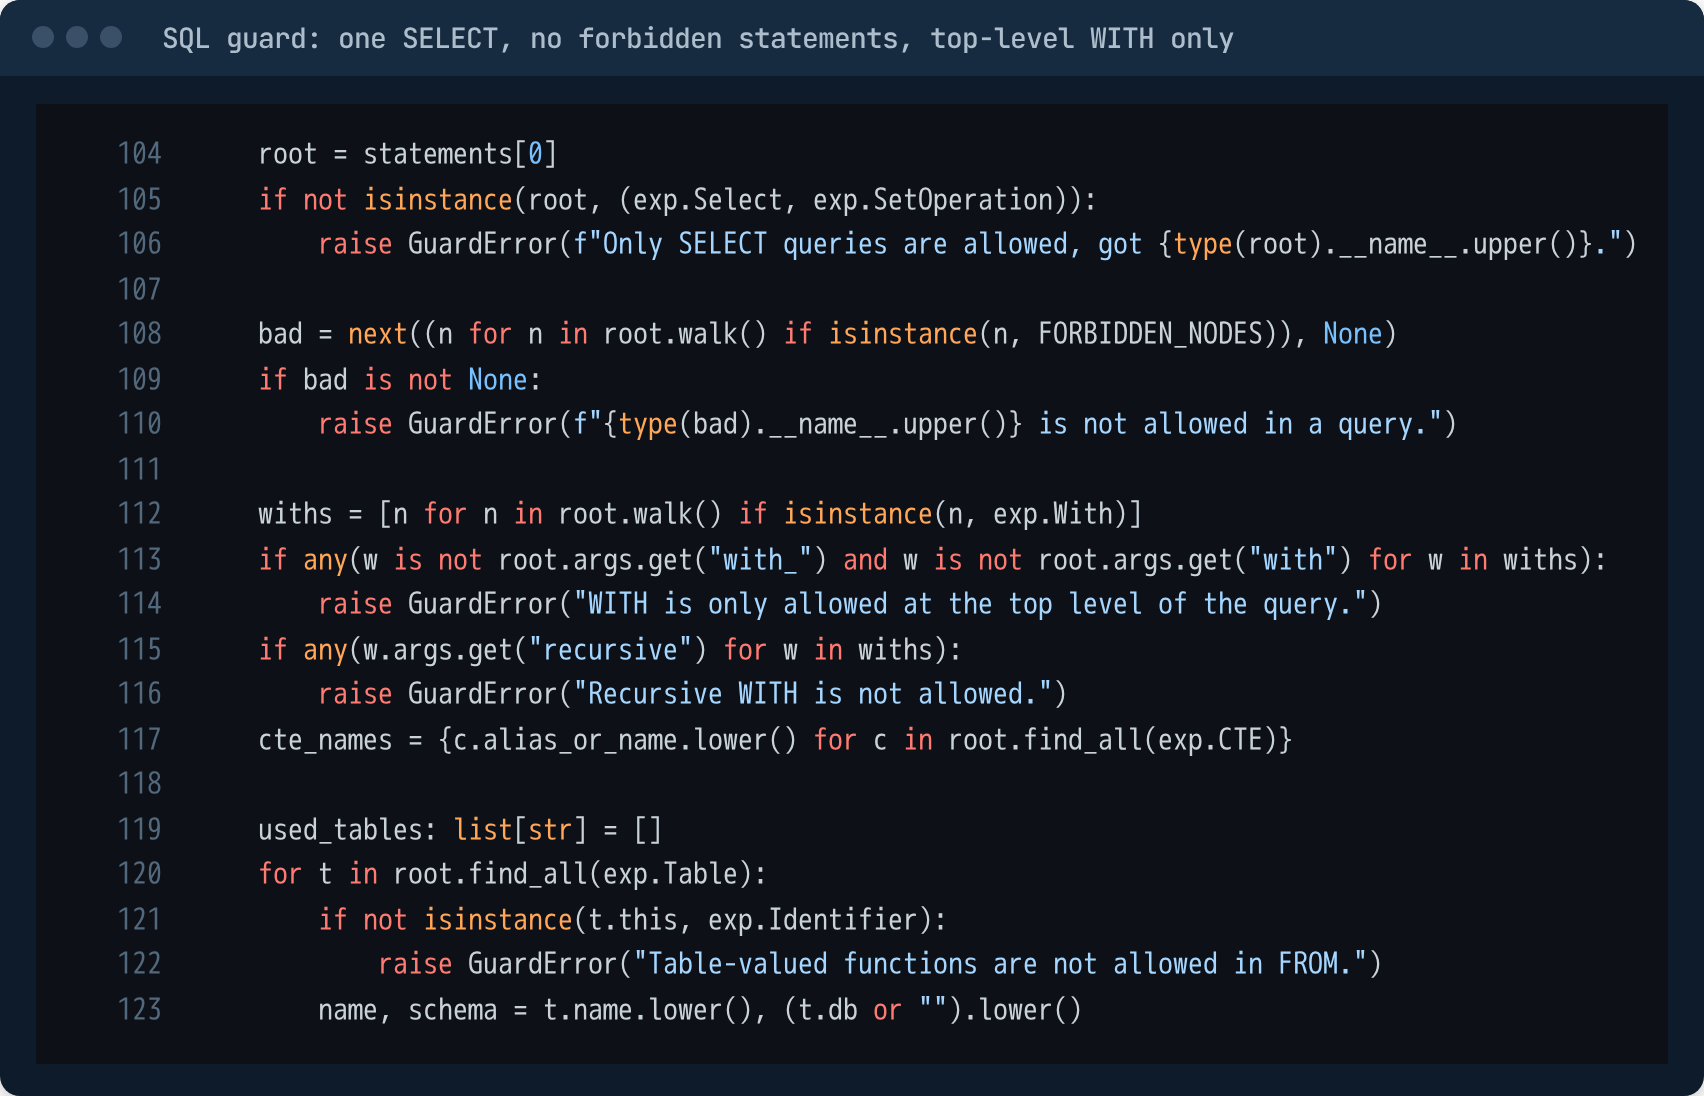
\includegraphics[width=0.85\textwidth]{code-guard-1.png}
\end{center}

\begin{keyconcept}
46 hostile queries were each refused \emph{for the intended reason}. Realistic questions plan under 5,000, while a telemetry self-join plans at 515 million and is refused before running.
\end{keyconcept}

% ====================================================================
\section{Results}
\subsection{Storage}
\begin{table}[h]
\centering
\begin{tabular}{lrr}
\toprule
Representation (70.7 M rows) & Size & Bytes per row\\
\midrule
PostgreSQL rowstore + index & 12,459 MB & 176.2\\
TimescaleDB columnstore & 385 MB & 5.4\\
Parquet (zstd, sorted) & 392 MB & 5.5\\
DuckDB native file & 700 MB & 9.9\\
\bottomrule
\end{tabular}
\caption{The columnstore is 32$\times$ smaller than the rowstore, and results matched the Parquet source.}
\end{table}

\subsection{Columnstore design experiment}
\begin{table}[h]
\centering
\small
\begin{tabular}{lrrrrr}
\toprule
Variant & Size & Q1 & Q2 & Q3 & Q4\\
\midrule
rowstore + B-tree & 3,631 MB & 10.8 ms & 1,519 ms & 65 ms & 246 ms\\
segment (flight, signal), order ts & 147 MB & 12.3 & 16 & 10.8 & 2.7\\
segment flight only & 149 MB & 12.9 & 18.0 & 11.6 & 3.2\\
segment signal only & 154 MB & 13.0 & 20.3 & 14.1 & 2.2\\
no segmentby & 157 MB & 15.0 & 29.7 & 13.7 & 3.6\\
1-day chunks & 150 MB & 16.3 & 15.3 & 12.3 & 3.4\\
30-day chunks & 143 MB & 9.2 & 8.3 & 5.7 & 2.4\\
\bottomrule
\end{tabular}
\caption{100 flights, 26.9 M rows, median of 7 warm runs. Q1 one signal of one flight; Q2 one signal across all flights; Q3 every signal of one flight; Q4 one signal in a 90-day window.}
\end{table}

\subsection{TimescaleDB against DuckDB}
\begin{table}[h]
\centering
\small
\begin{tabular}{lrrr}
\toprule
Query (p50, ms) & Timescale columnstore & DuckDB over Parquet & DuckDB native\\
\midrule
Q1 one signal, one flight, 1 s buckets & 25.4 & 25.3 & 4.9\\
Q2 one signal, all flights & 69.2 & 30.6 & 12.9\\
Q3 every signal of one flight & 18.7 & 45.7 & 22.5\\
Q4 one signal, 90-day window & 3.8 & 28.4 & 4.5\\
Q5 count and mean per signal, all data & 811.8 & 1,057.8 & 478.3\\
Q6 min/max/mean per flight and signal & 1,007.5 & 2,605.3 & 2,004.0\\
\bottomrule
\end{tabular}
\caption{70,731,891 rows, median of 5 warm runs. Load: Timescale \code{COPY} 286,792 rows/s; DuckDB bulk insert from Parquet 6,153,564 rows/s; DuckDB row-by-row insert 603 rows/s.}
\end{table}

\subsection{Vector indexes}
\begin{table}[h]
\centering
\small
\begin{tabular}{lrrrr}
\toprule
Index (100,000 vectors) & Build & Size & p50 at recall $\ge$ 0.95 & $\ge$ 0.99\\
\midrule
HNSW m=16 & 56 s & 819 MB & 2.7 ms & not reached\\
HNSW m=32 & 149 s & 819 MB & 2.4 ms & 3.2 ms\\
IVFFlat, 316 lists & 17 s & 822 MB & 5.5 ms & 9.3 ms\\
IVFFlat, 100 lists & 8.5 s & 820 MB & 8.4 ms & 14.8 ms\\
DiskANN & 268 s & 68 MB & not reached & not reached (max 0.74)\\
\bottomrule
\end{tabular}
\caption{1,536 dimensions, 200 queries, top 10; exact search takes 362 ms.}
\end{table}

A controlled 50,000-vector comparison at two noise levels (relative contrast 6.0 and 2.0, the real corpus being 20.5) left the ranking unchanged: HNSW m=32 was fastest at recall 0.99 in both, and DiskANN peaked at 0.845 and 0.889 recall.

\subsection{Filtered search}
\begin{table}[h]
\centering
\small
\begin{tabular}{lcccc}
\toprule
Strategy (rows returned of 10) & keeps 0.1\% & 1\% & 10\% & 50\%\\
\midrule
HNSW post-filter, ef 40 & 0.0 & 0.4 & 4.1 & 10\\
HNSW post-filter, ef 400 & 0.3 & 4.2 & 10 & 10\\
HNSW iterative scan & 10 & 10 & 10 & 10\\
B-tree filter, exact sort & 10 & 10 & 10 & 10\\
\bottomrule
\end{tabular}
\caption{Exact sort takes 1.0, 7.0, 55 and 329 ms at the four selectivities; iterative scan takes 50, 6.8, 2.3 and 1.8 ms. Crossover near 1,000 rows.}
\end{table}

\subsection{Search quality and natural-language SQL}
\begin{table}[h]
\centering
\begin{tabular}{lrr}
\toprule
Search method (65 queries) & nDCG@10 & hard paraphrases\\
\midrule
vector only & 0.710 & 0.59\\
vector + light full text (0.1) & 0.709 & 0.59\\
plain RRF & 0.600 & 0.43\\
full text only & 0.48 & 0.31\\
\bottomrule
\end{tabular}
\caption{Plain fusion is worse than vector only: paired difference $-0.109$, 95\% CI $[-0.172,-0.051]$.}
\end{table}

\begin{table}[h]
\centering
\begin{tabular}{lr}
\toprule
NL-to-SQL condition (27 held-out questions) & Strict execution accuracy\\
\midrule
semantic views & 0.89\\
raw tables + same documentation & 0.70\\
raw tables alone & 0.26\\
\bottomrule
\end{tabular}
\caption{Documentation: 0.26 to 0.70, 12 questions gained and none lost ($p=0.0005$). Views add 0.19 more (6 gained, 1 lost, $p=0.125$, not significant).}
\end{table}

\begin{insight}
Without documentation the model rarely failed loudly: 17 of 27 answers were confident and wrong. It never fabricated an answer to an unanswerable question.
\end{insight}

\subsection{The application}
\begin{figure}[h]
\centering
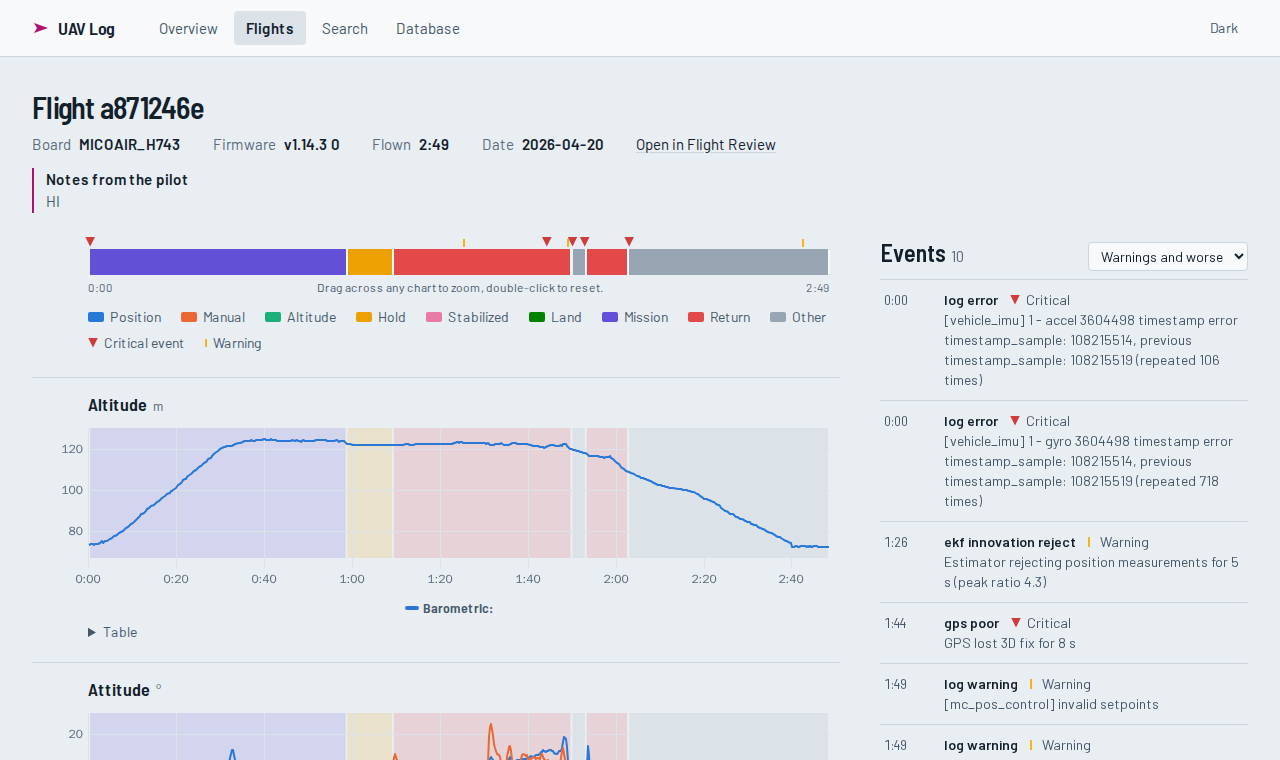
\includegraphics[width=0.48\textwidth]{crop-flight-light-1280.png}\hfill
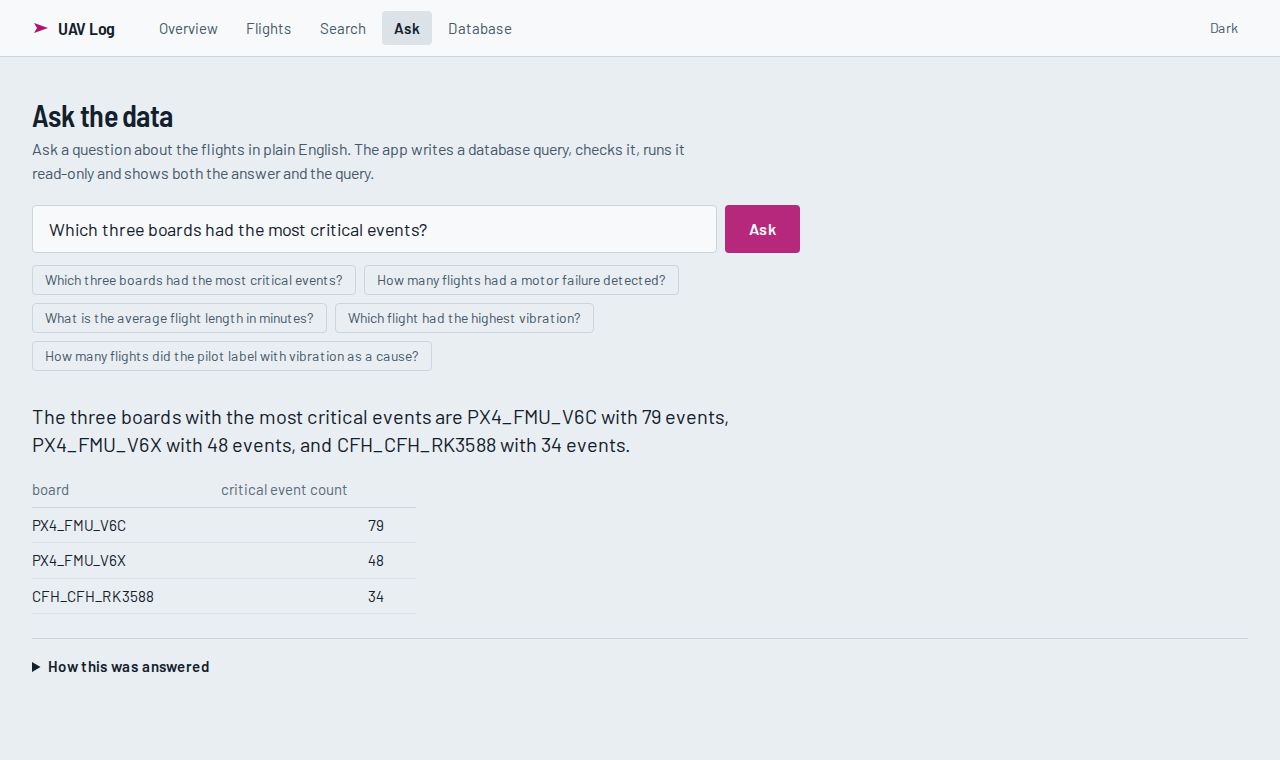
\includegraphics[width=0.48\textwidth]{crop-ask-light-1280.png}
\caption{A flight (mode ribbon, min/max envelopes, events) and the Ask page (generated SQL, cost, guard actions).}
\end{figure}

% ====================================================================
\section{Theoretical Comparison Table}
\begin{table}[h]
\centering
\small
\renewcommand{\arraystretch}{1.25}
\begin{tabular}{p{2.7cm}p{3.1cm}p{3.1cm}p{3.6cm}}
\toprule
Choice & Strength & Weakness & Used here for\\
\midrule
Rowstore + B-tree & Fast point reads, simple & 176 B/row, slow scans & Baseline\\
Columnstore & 32$\times$ smaller, pruned reads & Updates cost more & Telemetry\\
DuckDB / Parquet & Fast scans, no server & Single writer, no roles & Comparator\\
HNSW & Fastest queries at high recall & Slow build, large & Event search\\
IVFFlat & Fast build & Slower queries & Comparator\\
DiskANN & 12$\times$ smaller & Lower recall here & Comparator\\
Post-filter & Simple & Under-returns & Avoided\\
Iterative scan & Restores row count & 50 ms at 0.1\% & Large filters\\
Exact sort & Exact, cheap if selective & Linear in matches & Selective filters\\
\bottomrule
\end{tabular}
\caption{Design alternatives and where each was used.}
\end{table}

% ====================================================================
\section{Glossary}
\begin{description}
  \item[Hypertable] Time-partitioned table in TimescaleDB.
  \item[Chunk] One time-range partition of a hypertable.
  \item[Columnstore] Compressed column-wise storage of old chunks.
  \item[Continuous aggregate] Incrementally maintained rollup (here 1-second min, max, mean).
  \item[Embedding] A list of numbers representing meaning; here 1,536 dimensions for events, 32 for flight signatures.
  \item[HNSW / IVFFlat / DiskANN] Approximate nearest-neighbour index families.
  \item[Recall@k] Fraction of the true top-$k$ returned.
  \item[nDCG@10] Ranking quality over the top 10, rewarding relevant results near the top.
  \item[RRF] Reciprocal rank fusion of several rankings.
  \item[Ontology] Concepts and relations; here stored in relational tables.
  \item[Gaps and islands] SQL pattern that finds runs of consecutive rows.
  \item[SKIP LOCKED] Row-locking mode that skips rows another transaction holds.
  \item[Idempotent] Safe to run twice with the same result.
  \item[Execution accuracy (EX)] Share of generated queries whose result equals the gold result.
  \item[RC10] Relative contrast of the 10th neighbour; lower means harder data.
  \item[Parquet] Open columnar file format.
\end{description}

% ====================================================================
\section{Frequently Asked Questions}
\paragraph{Why one database instead of several specialised ones?}
Transactions, roles, joins to the ontology and vectors then live together. DuckDB won some scans in the comparison but gives up concurrent writers and roles.

\paragraph{Is 300 flights enough?}
It is a stated limit. The storage results are measured on 70.7 million rows; vector benchmarks use 50,000 and 100,000 perturbed vectors. A large run on 10,000 or more logs is planned and every volume is configurable.

\paragraph{Why did hybrid search lose?}
On 65 queries vector similarity already handles paraphrases, and plain fusion lets weak keyword hits displace good vector hits. With a small keyword weight it ties; no evidence was found that it helps.

\paragraph{Is the NL-to-SQL ``safe''?}
It is defended in four independent layers and tested with 46 hostile queries. The remaining risk is correctness (confident wrong answers), which is why the SQL and cost are shown.

\paragraph{What is untested?}
The snapshot/restore script was deliberately left untested and is documented that way, and the large-scale run has not happened.

% ====================================================================
\section{Conclusions}
\begin{itemize}
  \item A single PostgreSQL instance can hold the time series, the ontology, the vectors and a guarded natural-language interface.
  \item Physical design reduced telemetry from 12.5 GB to 385 MB (32$\times$); measured, not assumed.
  \item For retrieval, filtering strategy mattered more than index choice, and a self-routing query beat any fixed plan.
  \item Documentation, more than views, drives NL-to-SQL accuracy; four independent layers make it safe.
  \item Limits: 300 flights, one machine, one model, author-written questions. Next: the large run, ArduPilot at scale, a concurrency benchmark.
\end{itemize}

\end{document}
